\fancyhead[C]{Section 16.1}
	\fancyhead[R]{\daytwentyone}

\iftoggle{questions}{
\begin{center}{\large \textbf{Math 2551 Worksheet: Scalar Line Integrals}}
\end{center}

\begin{enumerate}
	\item For each curve, find a parameterization of the curve with the specified orientation.
	\begin{enumerate}
		\item The line segment in $\R^3$ from $(0,1,-2)$ to $(3,-1,2)$.
		
		\item The line segment in $\R^3$ from $(3,-1,2)$ to $(0,1,-2)$.
		
		\item The circle of radius 3 in $\R^2$ centered at the origin, beginning at the point $(0,-3)$ and proceeding clockwise around the circle.
		
		\item In $\R^2$, the portion of the parabola $y^2=x$ from the point $(4,2)$ to the point $(1,-1)$.\\
	\end{enumerate}
	
	For problems 2 to 4 below, do the set up of each line integral before doing any computations.
	
	\item Find the line integral of $f(x,y,z):=\sqrt{x^2+y^2}$ over the curve 
	$\br(t)= \vecf{(-4\sin t)}{+(4\cos t)}{+3t},$ $t \in [0,2\pi]$.\\
	
	\item Find the line integral of $f(x, y) =\sqrt{4x+1}$ over $C$ where $C$ is the part of the curve $x=y^2$ from the point $(4, -2)$ to $(1, 1)$.\\
	
	
	\item Let $C$ be the curve with parameterization
	\[
	\br(t)=\vecf{(e^t \cos t)}{+(e^t\sin t)}{+e^t},\quad t \in [0,\pi].
	\]
	Find the mass of $C$ if the density of a wire along $C$ is $\delta(x,y,z)=z^{-1}$.\\
	
	
	
	\textbf{Vector Field Problems:} In Chapter 13, we talked about vector-valued functions: functions whose input is a single real number and whose output is a vector in $\R^2$ or $\R^3$.  A very important related type of function in this unit is a \textbf{vector field}, which is a function that takes a point $(x,y)$ in $\R^2$ and outputs a vector in $\R^2$ or a point $(x,y,z)$ in $\R^3$ and outputs a vector in $\R^3$.
	
	\item If we want to make a decision based on what the wind is doing, then we need to keep track of not just its strength at any point, but also its direction! So a vector field is a good model here: at each point $(x,y)$, we can record the velocity vector for the wind.
	
	Suppose that given the point $(x,y)$ in the plane, we know that the wind velocity at that point is given by the vector $\bF(x,y)=\langle y, x\rangle$.  For example, at the point $(1,-1)$, the wind velocity is $\bF(1,-1)=\langle -1,1\rangle$.  Fill in the table below with the wind velocity vectors for the given points.\\
	
	\begin{tabular}{c|c}
		$(x,y)$ & $(-2,0)\quad (-1,2)\quad (0,-2)\quad (1,1)\quad (2,3)\quad (3,2)\quad (-1,0)\quad (1,3)$ \\
		\hline $\bF(x,y)$ &
	\end{tabular}
	
	\pagebreak
	
	\item Another useful way of recording this information is to plot the velocity vectors!  At each point $(x,y)$ we will draw the vector $\bF(x,y)$ starting with the tail of the vector at $(x,y)$.  This has been done for you with the point $(1,-1)$ below.  Fill in the plot with the other vectors you found in the last problem.
	
	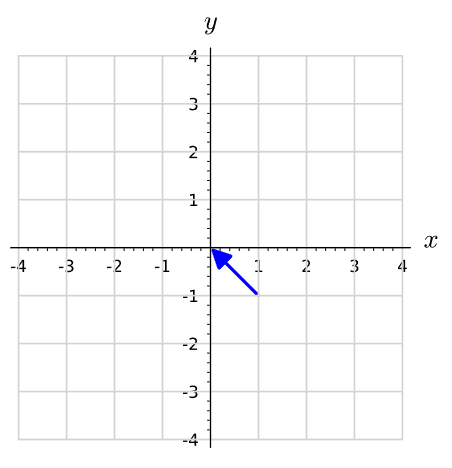
\includegraphics[scale=0.6]{ws_21_plot.png}
	
	CalcPlot3d can graph vector fields too! Use it to check your work and see the full detail of this vector field.
	
	
	\item Let $f(x,y)=\frac{1}{2}(x-y)^2$. Find the gradient vector field, $\nabla f$, of $f$ and sketch it.
\end{enumerate}
}{}

\iftoggle{answers}{
\begin{center}{\large \textbf{Math 2551 Worksheet Answers: Scalar Line Integrals}}
\end{center}
\begin{enumerate}
	\item There are many possible correct answers!  Here are some.
	\begin{enumerate}
		\item $\br(t)=\langle 3t, -2t+1, 4t-2\rangle, \quad 0\leq t \leq 1$
		
		\item  $\br(t)=\langle -3t+3, 2t-1, -4t+2\rangle, \quad 0\leq t \leq 1$
		
		\item $\br(t)=\langle 3 \sin(t), 3\cos(t) \rangle, \quad \pi\leq t\leq 3\pi$
		
		\item $\br(t)=\langle t^2, -t\rangle \quad -2 \leq t \leq 1$
	\end{enumerate}
	\item The integral to compute is $\Ds \int_0^{2\pi} 20\ dt$ since $f(\br(t))=4$ and $\|\br'(t)\|=5$.  Its value is $40 \pi$.
	
	\item The integral to compute is $Ds \int_{-2}^1 4t^2+1\ dt$. Its value is $15$.
	
	
	\item The integral to compute is $Ds \int_0^{\pi} e^{-t}e^t\sqrt{3}\ dt$ $\sqrt{3}\pi$
	
	
	\item	
	\begin{tabular}{c|c}
		$(x,y)$ & $(-2,0)\quad (-1,2)\quad (0,-2)\quad (1,1)\quad (2,3)\quad (3,2)\quad (-1,0)\quad (1,3)$ \\
		\hline $\bF(x,y)$ & $\langle 0, -2 \rangle\quad \langle 2,-1\rangle\quad \langle -2, 0 \rangle \quad \langle 1,1 \rangle \quad \langle 3,2 \rangle \quad \langle 2,3 \rangle \quad \langle 0, -1 \rangle \quad \langle 3, 1\rangle$
	\end{tabular}
	
	\item \begin{minipage}{0.5\textwidth}Without rescaling vectors to fit better:
		
		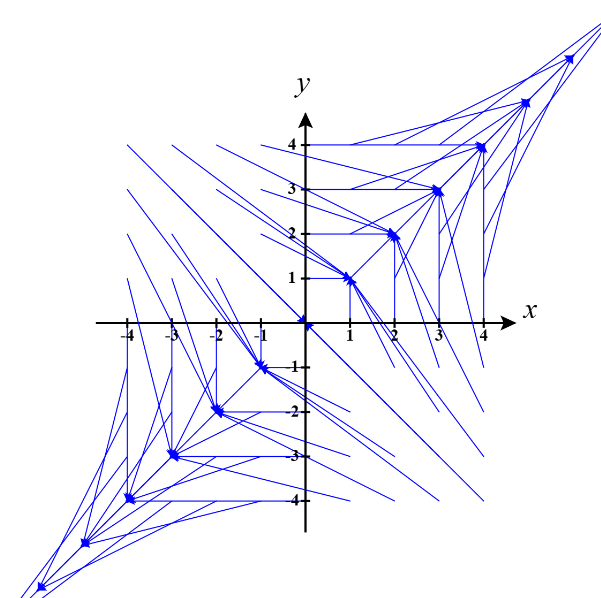
\includegraphics[scale=0.4]{ws_21_plot_ans_noscale.png}
	\end{minipage}\begin{minipage}{0.5\textwidth}
	With rescaling:
	
	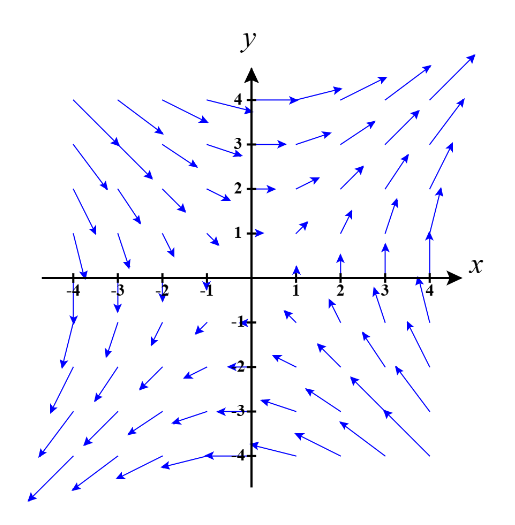
\includegraphics[scale=0.4]{ws_21_plot_ans.png}
\end{minipage}
	
	\item $\nabla f(x,y)=\langle x-y,y-x\rangle$
\end{enumerate}
}{}
\iftoggle{solutions}
{
Solutions go here in the same format.
}{}
